% Options for packages loaded elsewhere
\PassOptionsToPackage{unicode}{hyperref}
\PassOptionsToPackage{hyphens}{url}
\PassOptionsToPackage{dvipsnames,svgnames*,x11names*}{xcolor}
%
\documentclass[
  a4paper,
  oneside]{book}
\usepackage{lmodern}
\usepackage{setspace}
\usepackage{amsmath}
\usepackage{ifxetex,ifluatex}
\ifnum 0\ifxetex 1\fi\ifluatex 1\fi=0 % if pdftex
  \usepackage[T1]{fontenc}
  \usepackage[utf8]{inputenc}
  \usepackage{textcomp} % provide euro and other symbols
  \usepackage{amssymb}
\else % if luatex or xetex
  \usepackage{unicode-math}
  \defaultfontfeatures{Scale=MatchLowercase}
  \defaultfontfeatures[\rmfamily]{Ligatures=TeX,Scale=1}
\fi
% Use upquote if available, for straight quotes in verbatim environments
\IfFileExists{upquote.sty}{\usepackage{upquote}}{}
\IfFileExists{microtype.sty}{% use microtype if available
  \usepackage[]{microtype}
  \UseMicrotypeSet[protrusion]{basicmath} % disable protrusion for tt fonts
}{}
\makeatletter
\@ifundefined{KOMAClassName}{% if non-KOMA class
  \IfFileExists{parskip.sty}{%
    \usepackage{parskip}
  }{% else
    \setlength{\parindent}{0pt}
    \setlength{\parskip}{6pt plus 2pt minus 1pt}}
}{% if KOMA class
  \KOMAoptions{parskip=half}}
\makeatother
\usepackage{xcolor}
\IfFileExists{xurl.sty}{\usepackage{xurl}}{} % add URL line breaks if available
\IfFileExists{bookmark.sty}{\usepackage{bookmark}}{\usepackage{hyperref}}
\hypersetup{
  pdftitle={QRAP: an R package and Shiny app for interactive RNA sequencing data analysis},
  pdfauthor={Shixue Gou},
  colorlinks=true,
  linkcolor=Maroon,
  filecolor=Maroon,
  citecolor=Blue,
  urlcolor=Blue,
  pdfcreator={LaTeX via pandoc}}
\urlstyle{same} % disable monospaced font for URLs
\usepackage[left=3cm, right=3cm, top=2.5cm, bottom=2.5cm]{geometry}
\usepackage{color}
\usepackage{fancyvrb}
\newcommand{\VerbBar}{|}
\newcommand{\VERB}{\Verb[commandchars=\\\{\}]}
\DefineVerbatimEnvironment{Highlighting}{Verbatim}{commandchars=\\\{\}}
% Add ',fontsize=\small' for more characters per line
\usepackage{framed}
\definecolor{shadecolor}{RGB}{248,248,248}
\newenvironment{Shaded}{\begin{snugshade}}{\end{snugshade}}
\newcommand{\AlertTok}[1]{\textcolor[rgb]{0.94,0.16,0.16}{#1}}
\newcommand{\AnnotationTok}[1]{\textcolor[rgb]{0.56,0.35,0.01}{\textbf{\textit{#1}}}}
\newcommand{\AttributeTok}[1]{\textcolor[rgb]{0.77,0.63,0.00}{#1}}
\newcommand{\BaseNTok}[1]{\textcolor[rgb]{0.00,0.00,0.81}{#1}}
\newcommand{\BuiltInTok}[1]{#1}
\newcommand{\CharTok}[1]{\textcolor[rgb]{0.31,0.60,0.02}{#1}}
\newcommand{\CommentTok}[1]{\textcolor[rgb]{0.56,0.35,0.01}{\textit{#1}}}
\newcommand{\CommentVarTok}[1]{\textcolor[rgb]{0.56,0.35,0.01}{\textbf{\textit{#1}}}}
\newcommand{\ConstantTok}[1]{\textcolor[rgb]{0.00,0.00,0.00}{#1}}
\newcommand{\ControlFlowTok}[1]{\textcolor[rgb]{0.13,0.29,0.53}{\textbf{#1}}}
\newcommand{\DataTypeTok}[1]{\textcolor[rgb]{0.13,0.29,0.53}{#1}}
\newcommand{\DecValTok}[1]{\textcolor[rgb]{0.00,0.00,0.81}{#1}}
\newcommand{\DocumentationTok}[1]{\textcolor[rgb]{0.56,0.35,0.01}{\textbf{\textit{#1}}}}
\newcommand{\ErrorTok}[1]{\textcolor[rgb]{0.64,0.00,0.00}{\textbf{#1}}}
\newcommand{\ExtensionTok}[1]{#1}
\newcommand{\FloatTok}[1]{\textcolor[rgb]{0.00,0.00,0.81}{#1}}
\newcommand{\FunctionTok}[1]{\textcolor[rgb]{0.00,0.00,0.00}{#1}}
\newcommand{\ImportTok}[1]{#1}
\newcommand{\InformationTok}[1]{\textcolor[rgb]{0.56,0.35,0.01}{\textbf{\textit{#1}}}}
\newcommand{\KeywordTok}[1]{\textcolor[rgb]{0.13,0.29,0.53}{\textbf{#1}}}
\newcommand{\NormalTok}[1]{#1}
\newcommand{\OperatorTok}[1]{\textcolor[rgb]{0.81,0.36,0.00}{\textbf{#1}}}
\newcommand{\OtherTok}[1]{\textcolor[rgb]{0.56,0.35,0.01}{#1}}
\newcommand{\PreprocessorTok}[1]{\textcolor[rgb]{0.56,0.35,0.01}{\textit{#1}}}
\newcommand{\RegionMarkerTok}[1]{#1}
\newcommand{\SpecialCharTok}[1]{\textcolor[rgb]{0.00,0.00,0.00}{#1}}
\newcommand{\SpecialStringTok}[1]{\textcolor[rgb]{0.31,0.60,0.02}{#1}}
\newcommand{\StringTok}[1]{\textcolor[rgb]{0.31,0.60,0.02}{#1}}
\newcommand{\VariableTok}[1]{\textcolor[rgb]{0.00,0.00,0.00}{#1}}
\newcommand{\VerbatimStringTok}[1]{\textcolor[rgb]{0.31,0.60,0.02}{#1}}
\newcommand{\WarningTok}[1]{\textcolor[rgb]{0.56,0.35,0.01}{\textbf{\textit{#1}}}}
\usepackage{longtable,booktabs}
\usepackage{calc} % for calculating minipage widths
% Correct order of tables after \paragraph or \subparagraph
\usepackage{etoolbox}
\makeatletter
\patchcmd\longtable{\par}{\if@noskipsec\mbox{}\fi\par}{}{}
\makeatother
% Allow footnotes in longtable head/foot
\IfFileExists{footnotehyper.sty}{\usepackage{footnotehyper}}{\usepackage{footnote}}
\makesavenoteenv{longtable}
\usepackage{graphicx}
\makeatletter
\def\maxwidth{\ifdim\Gin@nat@width>\linewidth\linewidth\else\Gin@nat@width\fi}
\def\maxheight{\ifdim\Gin@nat@height>\textheight\textheight\else\Gin@nat@height\fi}
\makeatother
% Scale images if necessary, so that they will not overflow the page
% margins by default, and it is still possible to overwrite the defaults
% using explicit options in \includegraphics[width, height, ...]{}
\setkeys{Gin}{width=\maxwidth,height=\maxheight,keepaspectratio}
% Set default figure placement to htbp
\makeatletter
\def\fps@figure{htbp}
\makeatother
\setlength{\emergencystretch}{3em} % prevent overfull lines
\providecommand{\tightlist}{%
  \setlength{\itemsep}{0pt}\setlength{\parskip}{0pt}}
\setcounter{secnumdepth}{5}
\usepackage{booktabs}
\ifluatex
  \usepackage{selnolig}  % disable illegal ligatures
\fi
\usepackage[]{natbib}
\bibliographystyle{apalike}

\title{QRAP: an R package and Shiny app for interactive RNA sequencing data analysis}
\author{Shixue Gou}
\date{2022-12-05}

\begin{document}
\maketitle

{
\hypersetup{linkcolor=}
\setcounter{tocdepth}{2}
\tableofcontents
}
\setstretch{1.25}
\hypertarget{preface}{%
\chapter*{Preface}\label{preface}}
\addcontentsline{toc}{chapter}{Preface}

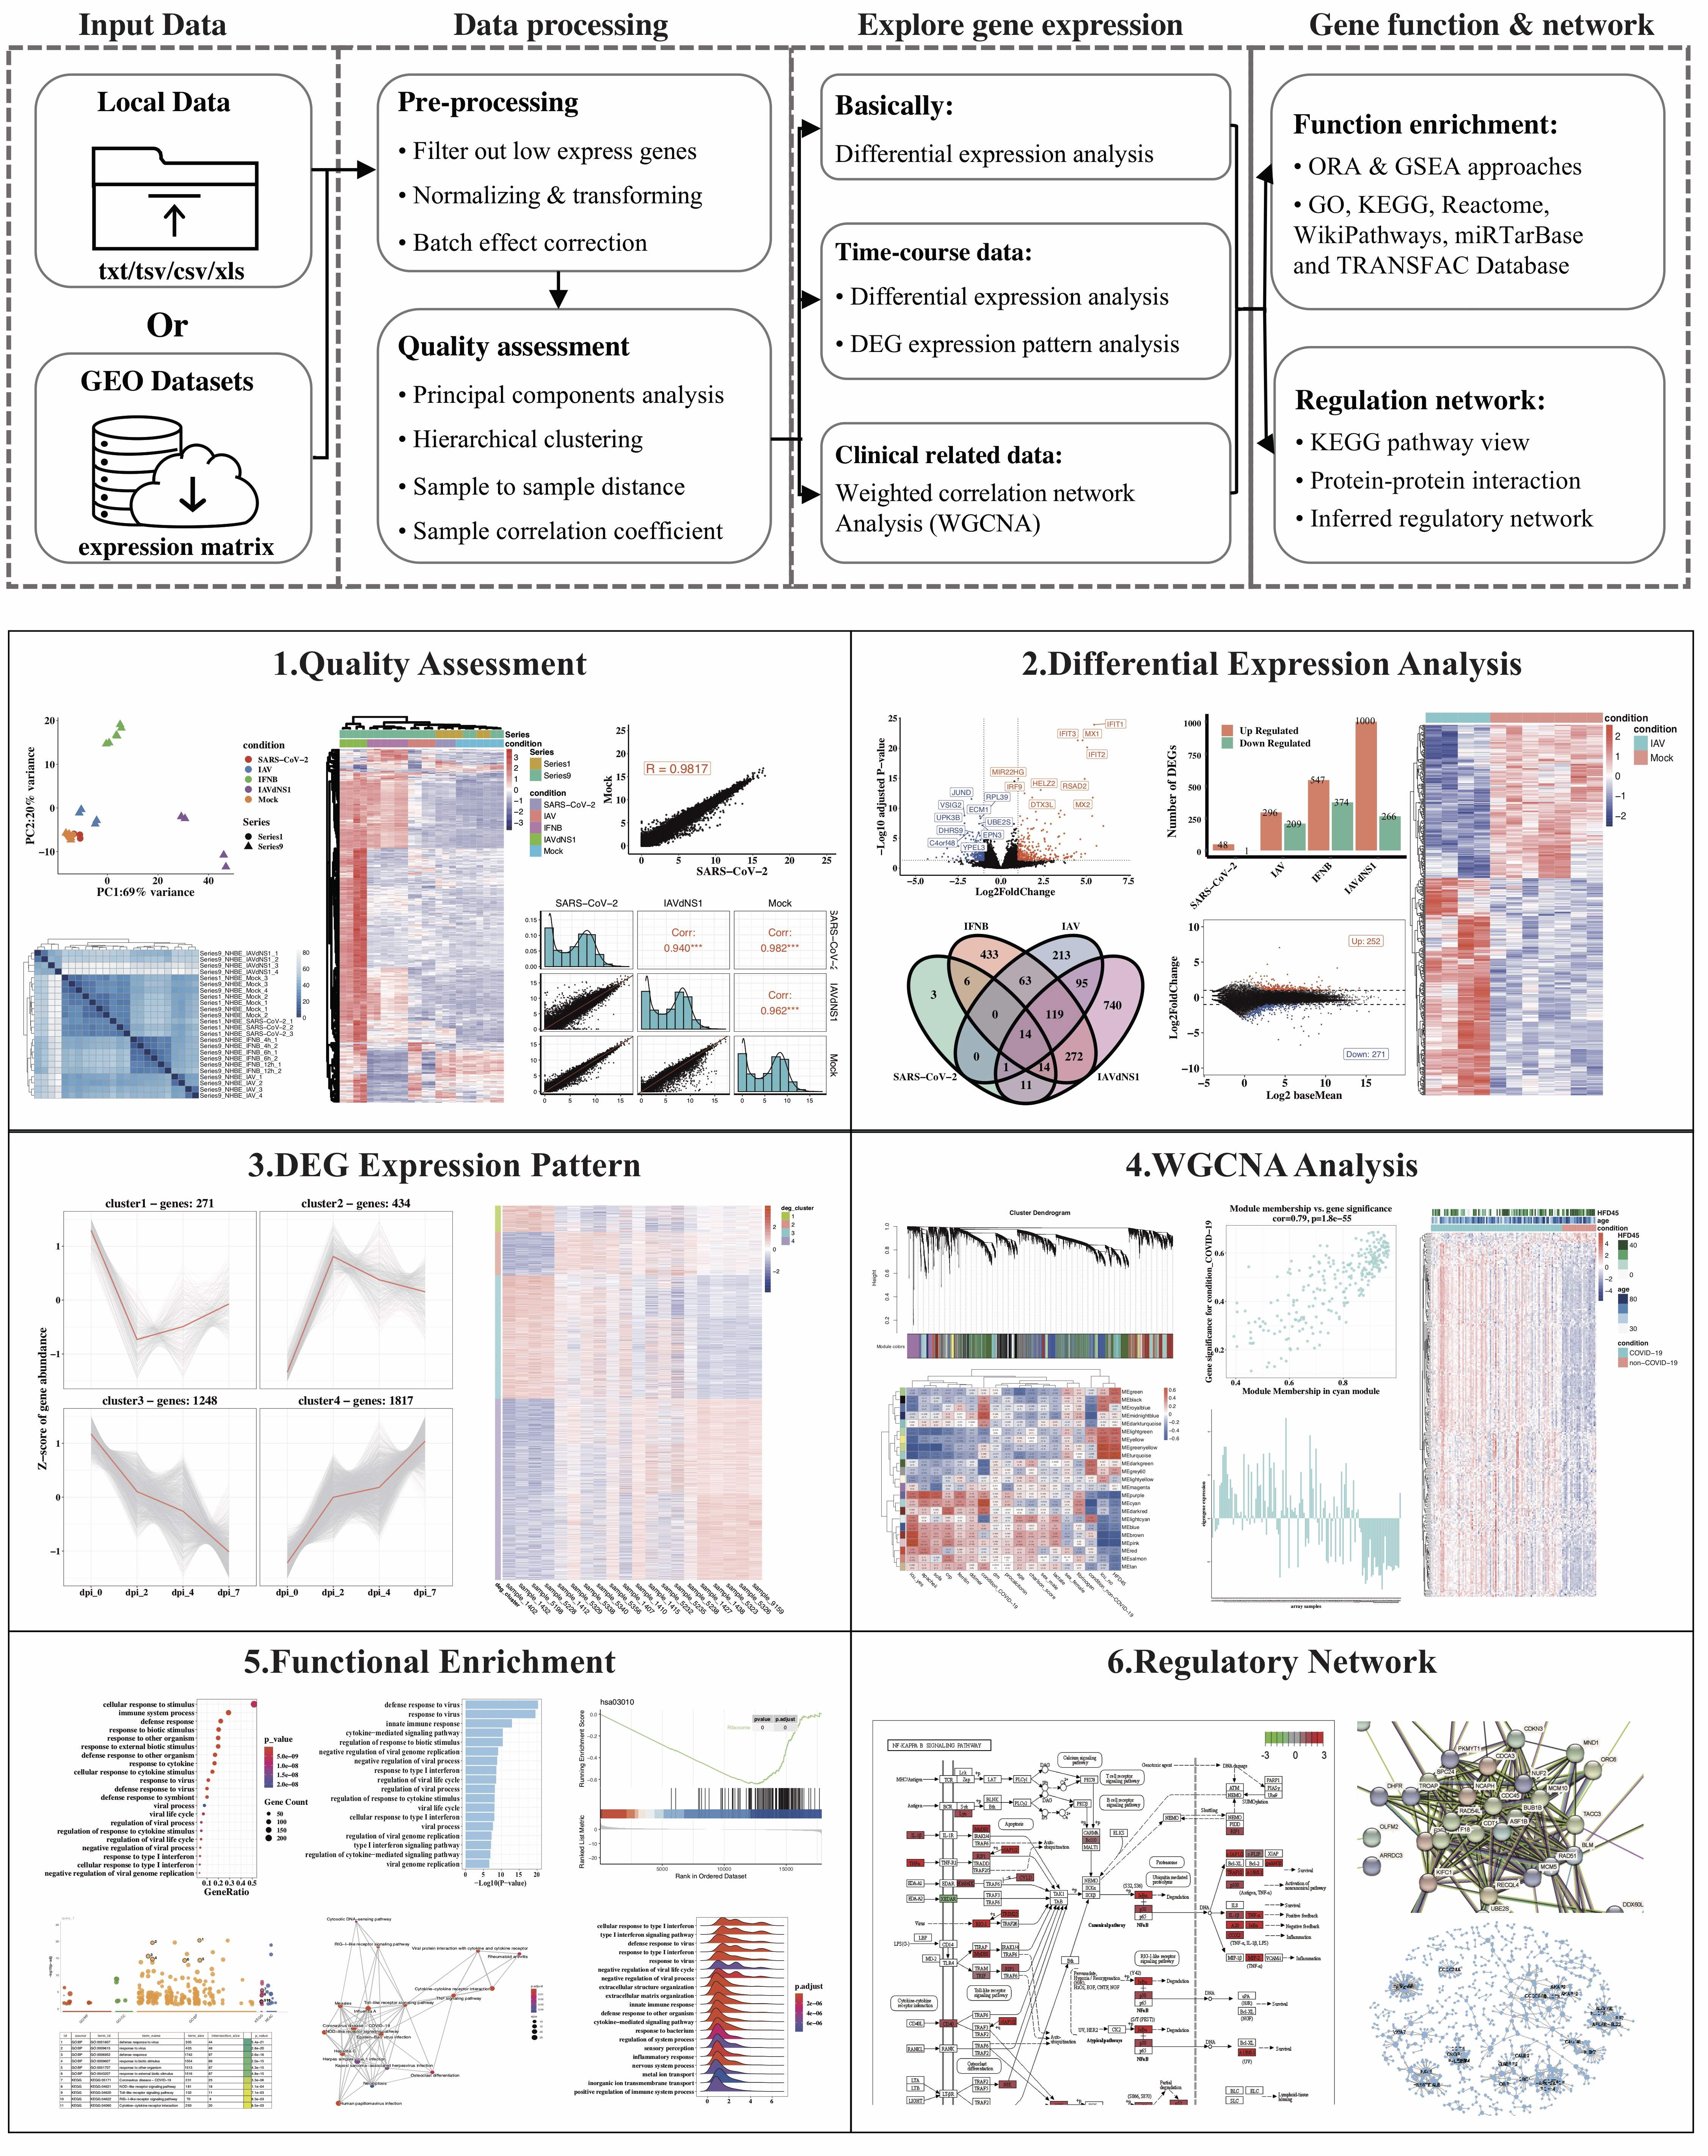
\includegraphics{images/workflow.jpg}

\hypertarget{intro}{%
\chapter{Introduction}\label{intro}}

\hypertarget{introduction}{%
\section{Introduction}\label{introduction}}

Motivation: RNA-sequencing (RNA-seq) has become the most commonly used tool in life science research for exploring whole transcript profiles. The advancement of next-generation sequencing has promoted a large amount of RNA-seq data. However, the popularity of bioinformatics lags far behind the generation of sequencing data, resulting in the inability of most researchers to analyze RNA-seq data. Although a large number of tools are currently available for RNA-seq analysis, data uploading, analysis, and visualization through an interactive interface are more acceptable to researchers than command-line codes.

Results: We designed an interactive RNA-seq analysis toolkit based on the R Shiny package, named QRAP (Quick RNA-seq Analysis Platform), which can easily accomplish RNA-seq data analysis and visualization through a user-friendly interface on the web page. As a comprehensive RNA-seq analysis tool, QRAP can support the analysis of publicly available and user-generated data, which include regular RNA-seq data, time-course RNA-seq data, and clinically relevant RNA-seq data, and provide functional annotation for approximately 500 species.

Availability and implementation: As an open source R package, QRAP can be freely accessed at \url{https://github.com/gsx-ucas/QRAP}.

\hypertarget{installation}{%
\section{Installation}\label{installation}}

\hypertarget{r-package}{%
\subsection{R package}\label{r-package}}

To install QRAP, R version 4.0 or greater is required. We also recommend installing R Studio.\\

\hypertarget{install-the-release-version-of-qrap}{%
\subsubsection{Install the release version of QRAP}\label{install-the-release-version-of-qrap}}

\begin{Shaded}
\begin{Highlighting}[]
\CommentTok{\# Enter commands in R (or R studio, if installed) }
\CommentTok{\# Install the remotes package install.packages(\textquotesingle{}devtools\textquotesingle{}) }
\NormalTok{devtools}\SpecialCharTok{::}\FunctionTok{install\_github}\NormalTok{(}\StringTok{"gsx{-}ucas/QRAP"}\NormalTok{)}
\end{Highlighting}
\end{Shaded}

\hypertarget{install-the-development-version-of-qrap}{%
\subsubsection{Install the development version of QRAP}\label{install-the-development-version-of-qrap}}

\begin{Shaded}
\begin{Highlighting}[]
\CommentTok{\# Enter commands in R (or R studio, if installed) }
\CommentTok{\# Install the remotes package install.packages(\textquotesingle{}devtools\textquotesingle{}) }
\NormalTok{devtools}\SpecialCharTok{::}\FunctionTok{install\_github}\NormalTok{(}\StringTok{"gsx{-}ucas/QRAP"}\NormalTok{, }\AttributeTok{ref =} \StringTok{"dev"}\NormalTok{)}
\end{Highlighting}
\end{Shaded}

\hypertarget{docker-image}{%
\subsection{Docker image}\label{docker-image}}

We provide docker images for QRAP via dockerhub. To pull the latest image using the command line:

\begin{Shaded}
\begin{Highlighting}[]
\CommentTok{\# Enter commands in shell}
\NormalTok{docker pull goushixue}\SpecialCharTok{/}\NormalTok{qrap}\SpecialCharTok{:}\NormalTok{latest}
\end{Highlighting}
\end{Shaded}

\hypertarget{get-started}{%
\section{Get started}\label{get-started}}

\hypertarget{launch-the-qrap-application-in-r-or-rstudio}{%
\subsection{Launch the QRAP application in R or Rstudio}\label{launch-the-qrap-application-in-r-or-rstudio}}

\begin{Shaded}
\begin{Highlighting}[]
\FunctionTok{library}\NormalTok{(QRAP) }\CommentTok{\# loading the QRAP library to R environment}
\FunctionTok{startQRAP}\NormalTok{() }\CommentTok{\# launch the QRAP application to web browser}
\end{Highlighting}
\end{Shaded}

Then you would get the link to activate your browser:\\
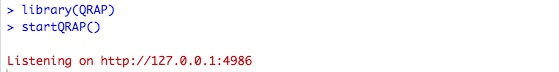
\includegraphics{images/launch_R.jpeg}\\
Use the link \url{http://127.0.0.1:4986} to access the interactive analysis interface. Note that the port (4986) should change to yours.\\

\hypertarget{launch-the-qrap-application-by-docker-image-in-shell}{%
\subsection{Launch the QRAP application by docker image in shell}\label{launch-the-qrap-application-by-docker-image-in-shell}}

\begin{Shaded}
\begin{Highlighting}[]
\NormalTok{docker run  }\SpecialCharTok{{-}}\NormalTok{p }\DecValTok{3838}\SpecialCharTok{:}\DecValTok{3838}\NormalTok{ goushixue}\SpecialCharTok{/}\NormalTok{qrap }\CommentTok{\# use the 3838 port }
\end{Highlighting}
\end{Shaded}

Then you would get the output like this:\\
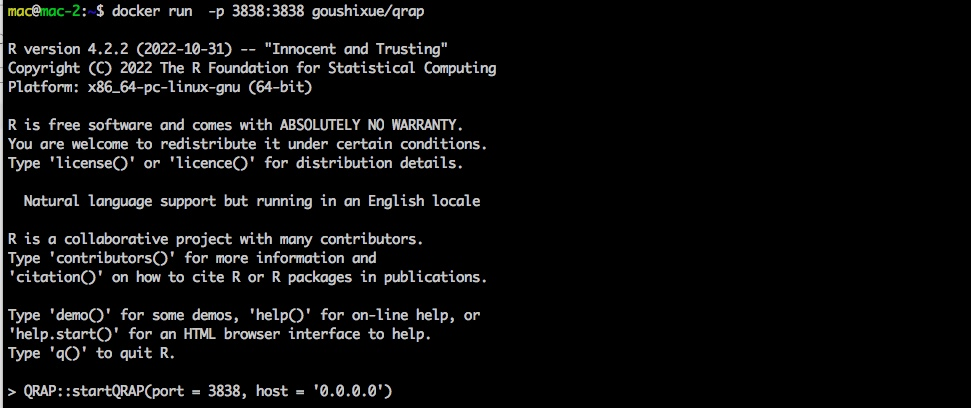
\includegraphics{images/launch_docker.jpeg}\\
Use the link \url{http://localhost:3838/} to access the interactive analysis interface.\\

\hypertarget{access-the-interactive-analysis-interface}{%
\subsection{Access the interactive analysis interface}\label{access-the-interactive-analysis-interface}}

Just start your analysis by clicking, clicking, clicking\ldots{}\\
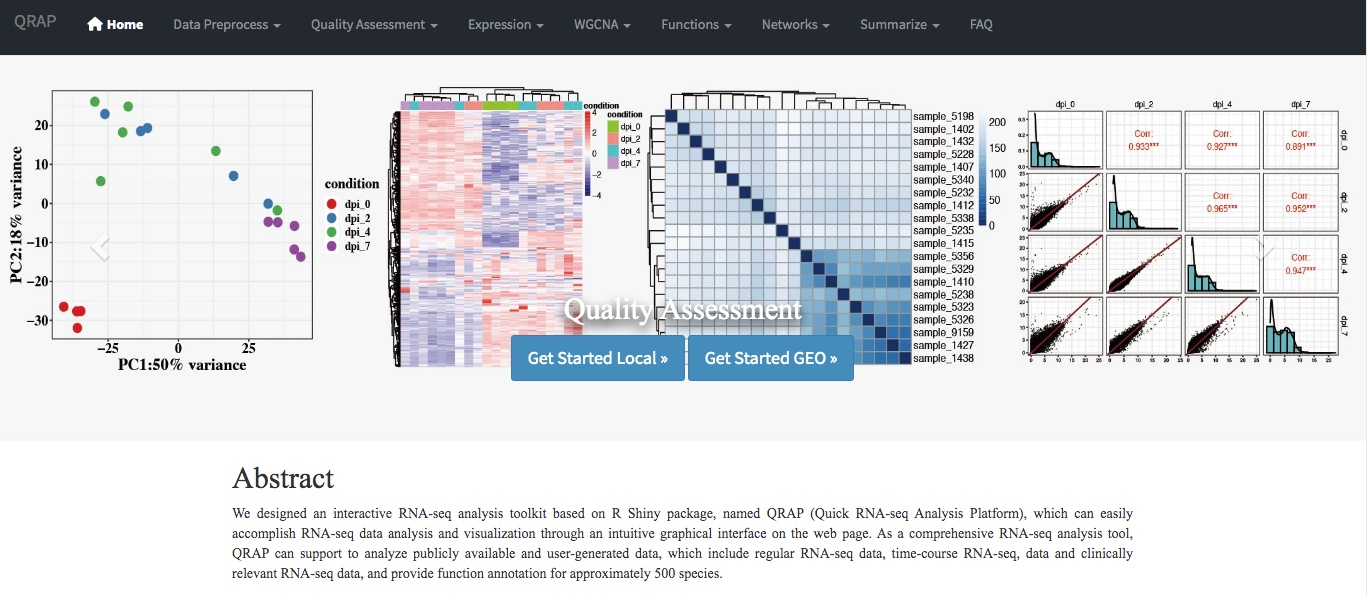
\includegraphics{images/launch_interface.jpeg}\\

\hypertarget{data-input-and-pre-processing}{%
\chapter{Data input and pre-processing}\label{data-input-and-pre-processing}}

\hypertarget{data-input}{%
\section{Data input}\label{data-input}}

QRAP can support to analyze publicly available and user-generated data. There are two action buttons, `Get Started Local' and `Get Started GEO', can activate corresponding data upload and processing pipeline.

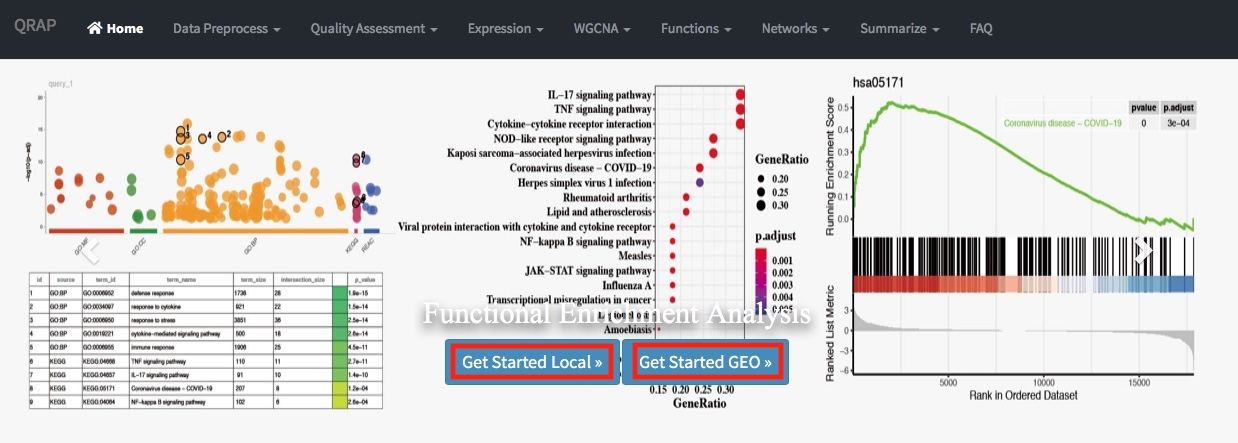
\includegraphics{images/start_button.jpeg}

\hypertarget{upload-local-file}{%
\subsection{Upload local file}\label{upload-local-file}}

For user generated local files, click the `Get Started Local' button to enter the data upload page.

\textbf{\emph{Parameters in this section:}}\\
- Choose input file: browser and upload the expression matrix file, accept .csv/.tsv/.tab/.txt format.\\
- First row as header ? This means use the first row of the expression matrix as column names, often is samples names.\\
- First column as rownames ? This means use the first column of the expression matrix as row names, often is gene names.\\

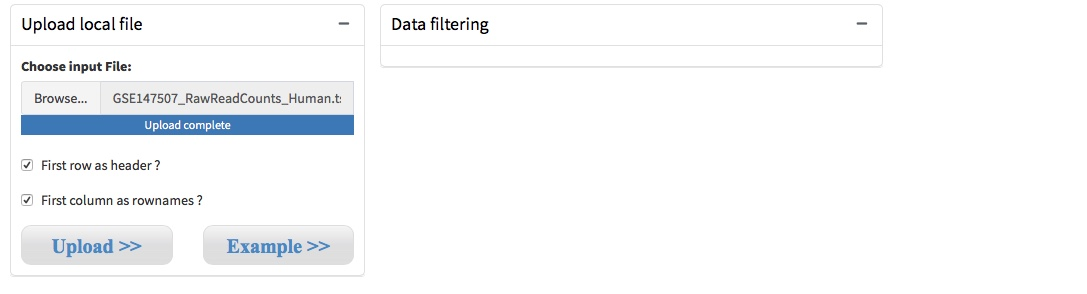
\includegraphics{images/upload_local_file.jpeg}

After select the local files and set the parameters, click the `Upload' button to preview the expression matrix.

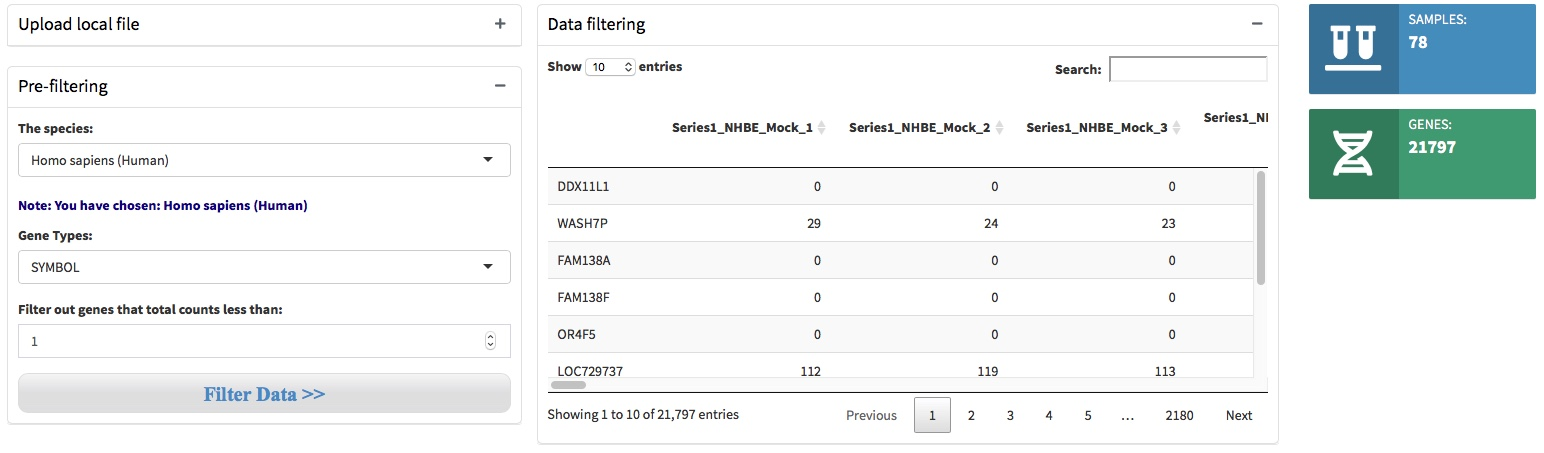
\includegraphics{images/local_expression_preview.jpeg}

Click `Example' will upload the example dataset internal, transcriptomes of SARS-Cov-2 infected normal human bronchial epithelial cells (GSE147507).

\hypertarget{pull-down-geo-datasets}{%
\subsection{Pull down GEO datasets}\label{pull-down-geo-datasets}}

The Gene Expression Omnibus (GEO) is a public repository that archives and freely distributes comprehensive sets of microarray, next-generation sequencing, and other forms of high-throughput functional genomic data submitted by the scientific community.

After you input the GEO Acession Number and active the `Download matrix' button, We will download the value matrix tables within GDSxxx or supplementary files within GSExxx, these files will store in the working directory of the R project you created.\\
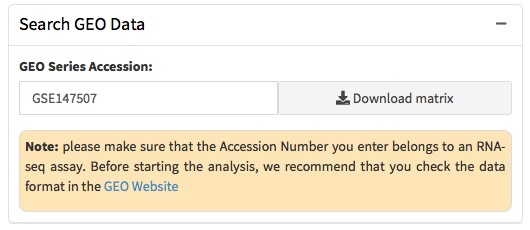
\includegraphics{images/search_geo_dataset.jpeg}\\

When the files download accomplished, there will show the download files name in the Parameter setting panel, and you should select file(s) that contain interested gene expression matrix and active the `Loading GEO' button to preview the matrix.\\
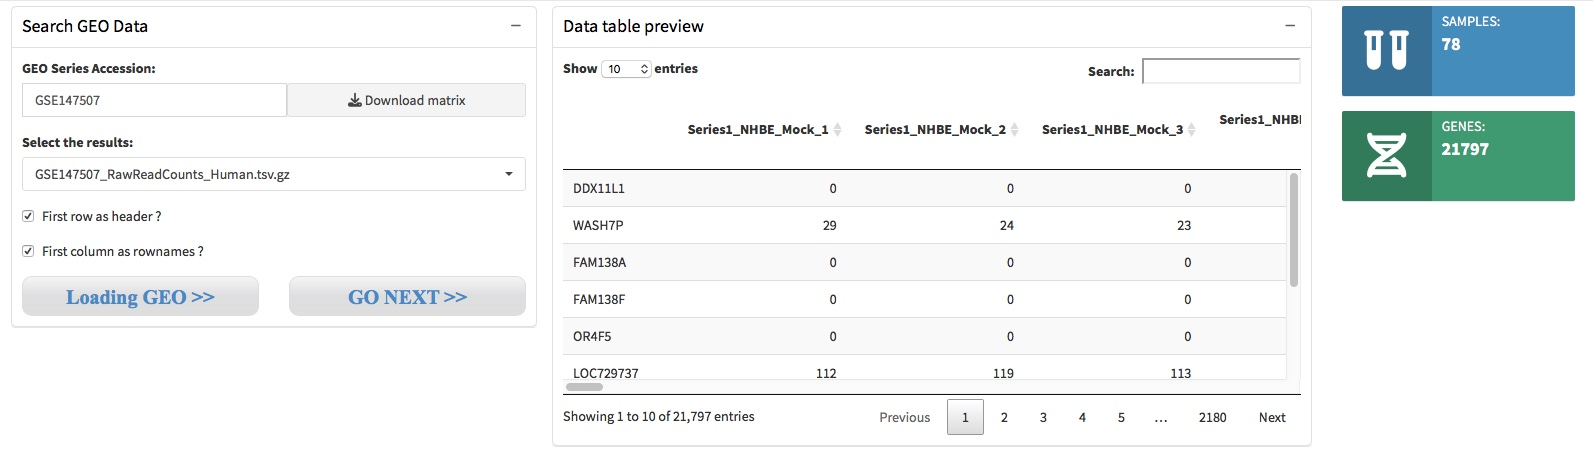
\includegraphics{images/geo_preview_single.jpeg}\\
Please Note that if the files are in a tar archive format, such as htseq-count generated results, these files will contain Gene ID and Gene Expression Value of each sample, respectively. Therefore, you need to provid the column number of the Gene ID and Gene Expression Value to help merge the files to generate an analysis ready gene expression matrix.

\begin{itemize}
\tightlist
\item
  Step 1. Choose a single file, and leave the `First row as header' and `First column as rownames' unchecked, then click the button `Loading GEO' to preview what the file contained.\\
  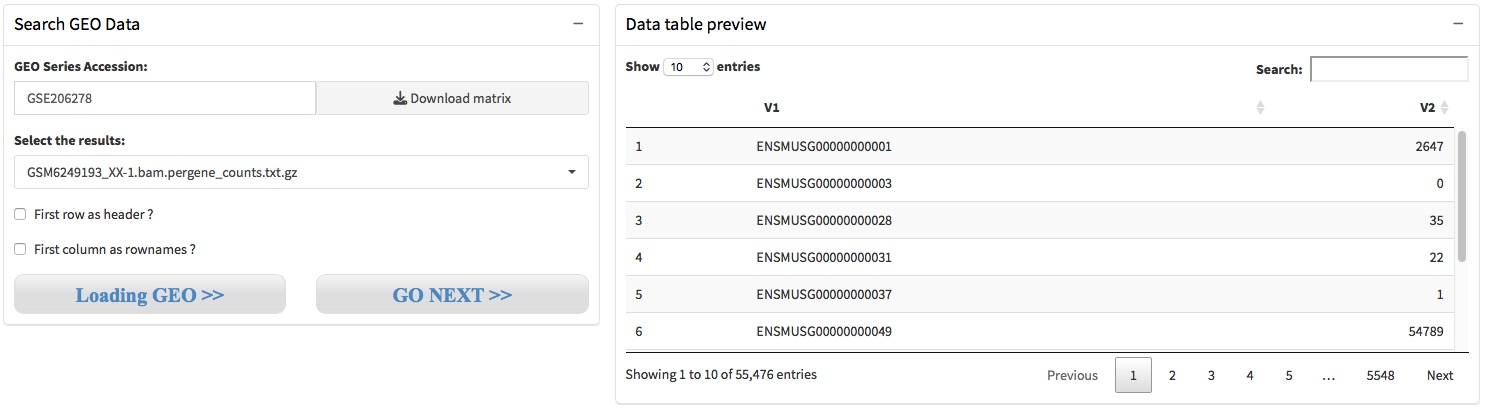
\includegraphics{images/geo_preview_multiple_setp1.jpeg}
\item
  Step 2. Choose all or interested files, set the column number of geneID and readCounts, then click the button `Loading GEO' to generate and preview the analysis ready expression matrix.\\
  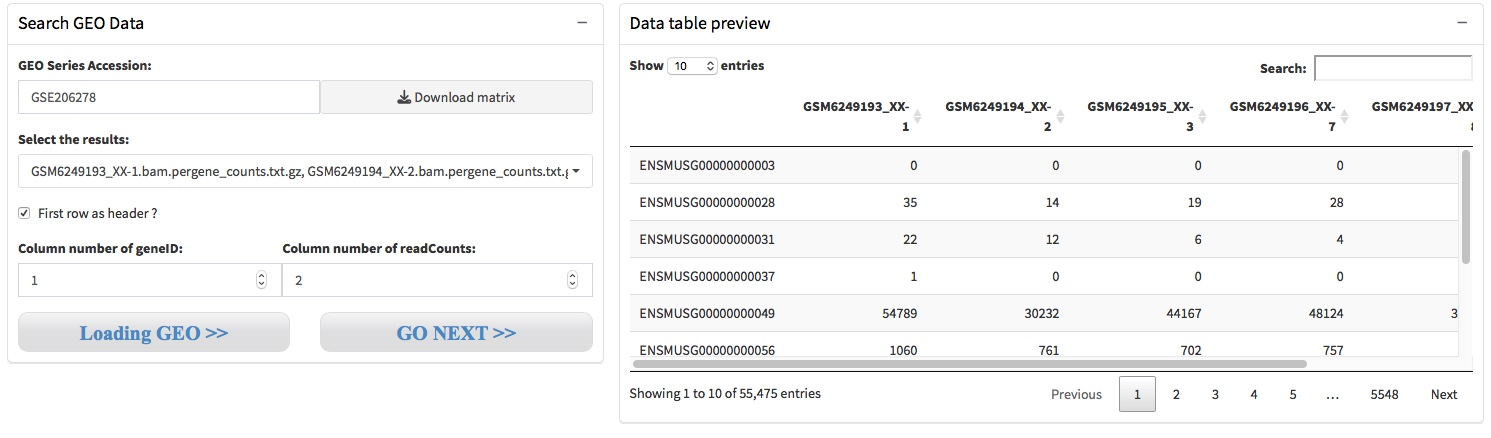
\includegraphics{images/geo_preview_multiple_setp2.jpeg}
\end{itemize}

\hypertarget{data-pre-processing}{%
\section{Data pre-processing}\label{data-pre-processing}}

QRAP starts with a read-counts matrix or GEO accession number, and then filters out low expression genes under an given threshold. We then specify the organisms and filtered out low expression genes.\\
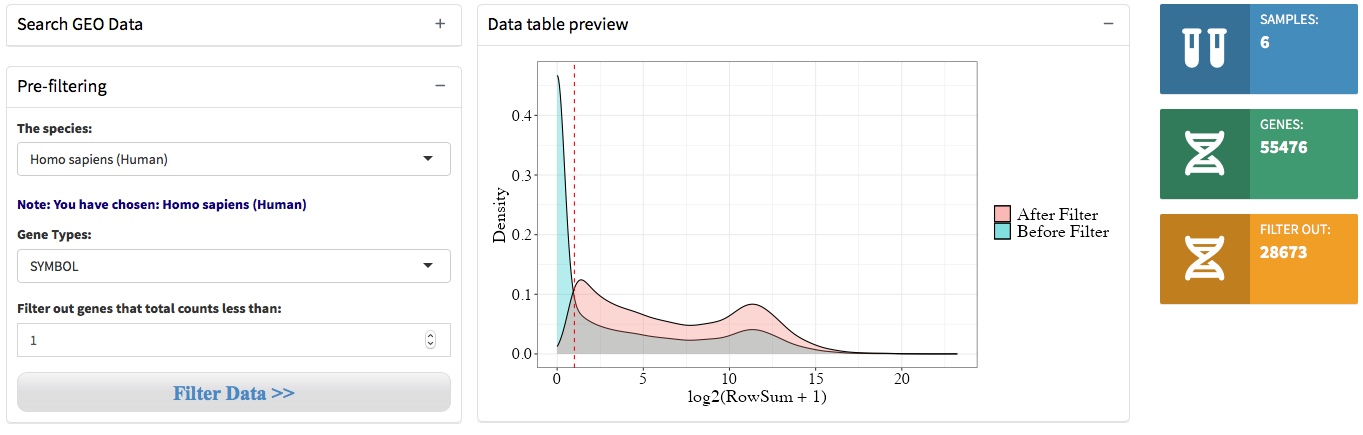
\includegraphics{images/prefiltering.jpeg}

\hypertarget{note-the-gene-types}{%
\subparagraph*{Note the Gene Types:}\label{note-the-gene-types}}
\addcontentsline{toc}{subparagraph}{Note the Gene Types:}

\begin{longtable}[]{@{}lll@{}}
\toprule
SYMBOL & ENSEMBL & ENTREZID\tabularnewline
\midrule
\endhead
GAPDH & ENSG00000111640 & 2597\tabularnewline
TP53 & ENSG00000141510 & 7157\tabularnewline
\bottomrule
\end{longtable}

\hypertarget{data-quality-exploring}{%
\chapter{Data quality exploring}\label{data-quality-exploring}}

We describe our methods in this chapter.

\hypertarget{principal-component-analysis-pca}{%
\section{principal component analysis (PCA)}\label{principal-component-analysis-pca}}

\hypertarget{hierarchical-clustering-heatmap}{%
\section{hierarchical clustering heatmap}\label{hierarchical-clustering-heatmap}}

\hypertarget{sample-to-sample-heatmap}{%
\section{sample-to-sample heatmap}\label{sample-to-sample-heatmap}}

\hypertarget{sample-correlation-coefficient}{%
\section{sample correlation coefficient}\label{sample-correlation-coefficient}}

\hypertarget{differential-expression-analysis}{%
\chapter{Differential expression analysis}\label{differential-expression-analysis}}

Some \emph{significant} applications are demonstrated in this chapter.

\hypertarget{extract-degs}{%
\section{Extract DEGs}\label{extract-degs}}

\hypertarget{visualize-degs}{%
\section{Visualize DEGs}\label{visualize-degs}}

\hypertarget{deg-expression-pattern-detection}{%
\chapter{DEG expression pattern detection}\label{deg-expression-pattern-detection}}

We have finished a nice book.

\hypertarget{detect-deg-expression-pattern}{%
\section{Detect DEG expression pattern}\label{detect-deg-expression-pattern}}

\hypertarget{visualize-deg-expression-pattern}{%
\section{Visualize DEG expression pattern}\label{visualize-deg-expression-pattern}}

\hypertarget{weighted-correlation-network-analysis}{%
\chapter{weighted correlation network analysis}\label{weighted-correlation-network-analysis}}

We have finished a nice book.

\hypertarget{data-preparation}{%
\section{Data preparation}\label{data-preparation}}

\hypertarget{soft-threshold-detection}{%
\section{Soft threshold detection}\label{soft-threshold-detection}}

\hypertarget{gene-module-detection}{%
\section{Gene module detection}\label{gene-module-detection}}

\hypertarget{module-traits-relationship}{%
\section{Module-Traits relationship}\label{module-traits-relationship}}

\hypertarget{mm-vs.-gs-scatterplot}{%
\section{MM vs.~GS scatterplot}\label{mm-vs.-gs-scatterplot}}

\hypertarget{module-gene-expression-visualization}{%
\section{Module gene expression visualization}\label{module-gene-expression-visualization}}

\hypertarget{functional-enrichment-analysis}{%
\chapter{functional enrichment analysis}\label{functional-enrichment-analysis}}

We have finished a nice book.

\hypertarget{gprofiler-api}{%
\section{Gprofiler API}\label{gprofiler-api}}

\hypertarget{clusterprofiler}{%
\section{ClusterProfiler}\label{clusterprofiler}}

\hypertarget{ora}{%
\subsection{ORA}\label{ora}}

\hypertarget{gsea}{%
\subsection{GSEA}\label{gsea}}

\hypertarget{gene-regulatory-network}{%
\chapter{Gene regulatory network}\label{gene-regulatory-network}}

We have finished a nice book.

\hypertarget{kegg-pathview}{%
\section{KEGG Pathview}\label{kegg-pathview}}

\hypertarget{ppi-network}{%
\section{PPI network}\label{ppi-network}}

\hypertarget{genie3-inffered-network}{%
\section{GENIE3 inffered network}\label{genie3-inffered-network}}

\hypertarget{summary-of-genes-and-functions}{%
\chapter{Summary of genes and functions}\label{summary-of-genes-and-functions}}

We have finished a nice book.

\hypertarget{summarize-genes}{%
\section{summarize genes}\label{summarize-genes}}

\hypertarget{summarize-functions}{%
\section{summarize functions}\label{summarize-functions}}

  \bibliography{book.bib,packages.bib}

\end{document}
